\documentclass{article}
\usepackage[utf8]{inputenc}

\title{Team 39: CS 184 Milestone}
\author{Yekang Chang, Jie Zeng, Liang Yang, Silu Chu}
% \date{April 2024}
\usepackage{hyperref}
\usepackage{listings}
\newcommand{\cmdname}[1]{\texttt{#1}}
\newcommand\footurl[1]{\footnote{\url{#1}}}
\newcommand\urllink[2]{#1\footurl{#2}}
\newcommand\foothref[3]{#1\footnote{\href{#2}{#3}}}
\usepackage{upquote}
\usepackage{graphicx} % For including graphics
\usepackage{subcaption} % For creating subfigures

\begin{document}

\maketitle
% summarize what you have accomplished, preliminary results, reflect on progress relative to your plan, and update your work plan as appropriate

The three-page slides are published at \url{https://drive.google.com/file/d/1w36IwNipihc5QhI1VJDkqmymObUJ4fVB/view?usp=sharing}, and the demo video link is published at \url{https://drive.google.com/file/d/1GqzvNQNkeHD_rDhUS0nEgtIZoKsKWUai/view?usp=sharing}.

\section{Summarization}

\hspace*{1em}In this project, our group will simulate the fluid within a tank, and then we will simulate the real-case scenario when a ball falls into and interacts with the fluid (which many liquid drops will bounce out). Currently, we have done a preliminary and basic implementation (in which some unreality will occur) for this scenario, including the demo for fluid (in the form of discrete liquid drops), as well as the preliminary simulation of the interaction after the ball drops and pluid particle splashed. 

\section{Preliminary Results}

\hspace*{1em}The below three figures are captured from our current preliminary simulation results. We have done a demo-simulation of the fluid. In this scenario, the fluid - simulated in the form of liquid drops, falls down from a "spawner" and spreads across the container tank. 

\noindent\hspace*{1em} We then do a preliminary simulation of the ball that falls into the pool and interacts with the liquid drops. Ball falls at different velocities will lead to different results of interaction with fluid. For example, when the ball falls from higher places or large velocity, more liquid drops will be splashed out, and will be splashed higher. 

\begin{figure}[h]
    \centering
    \begin{subfigure}[b]{0.33\textwidth}
        \centering
        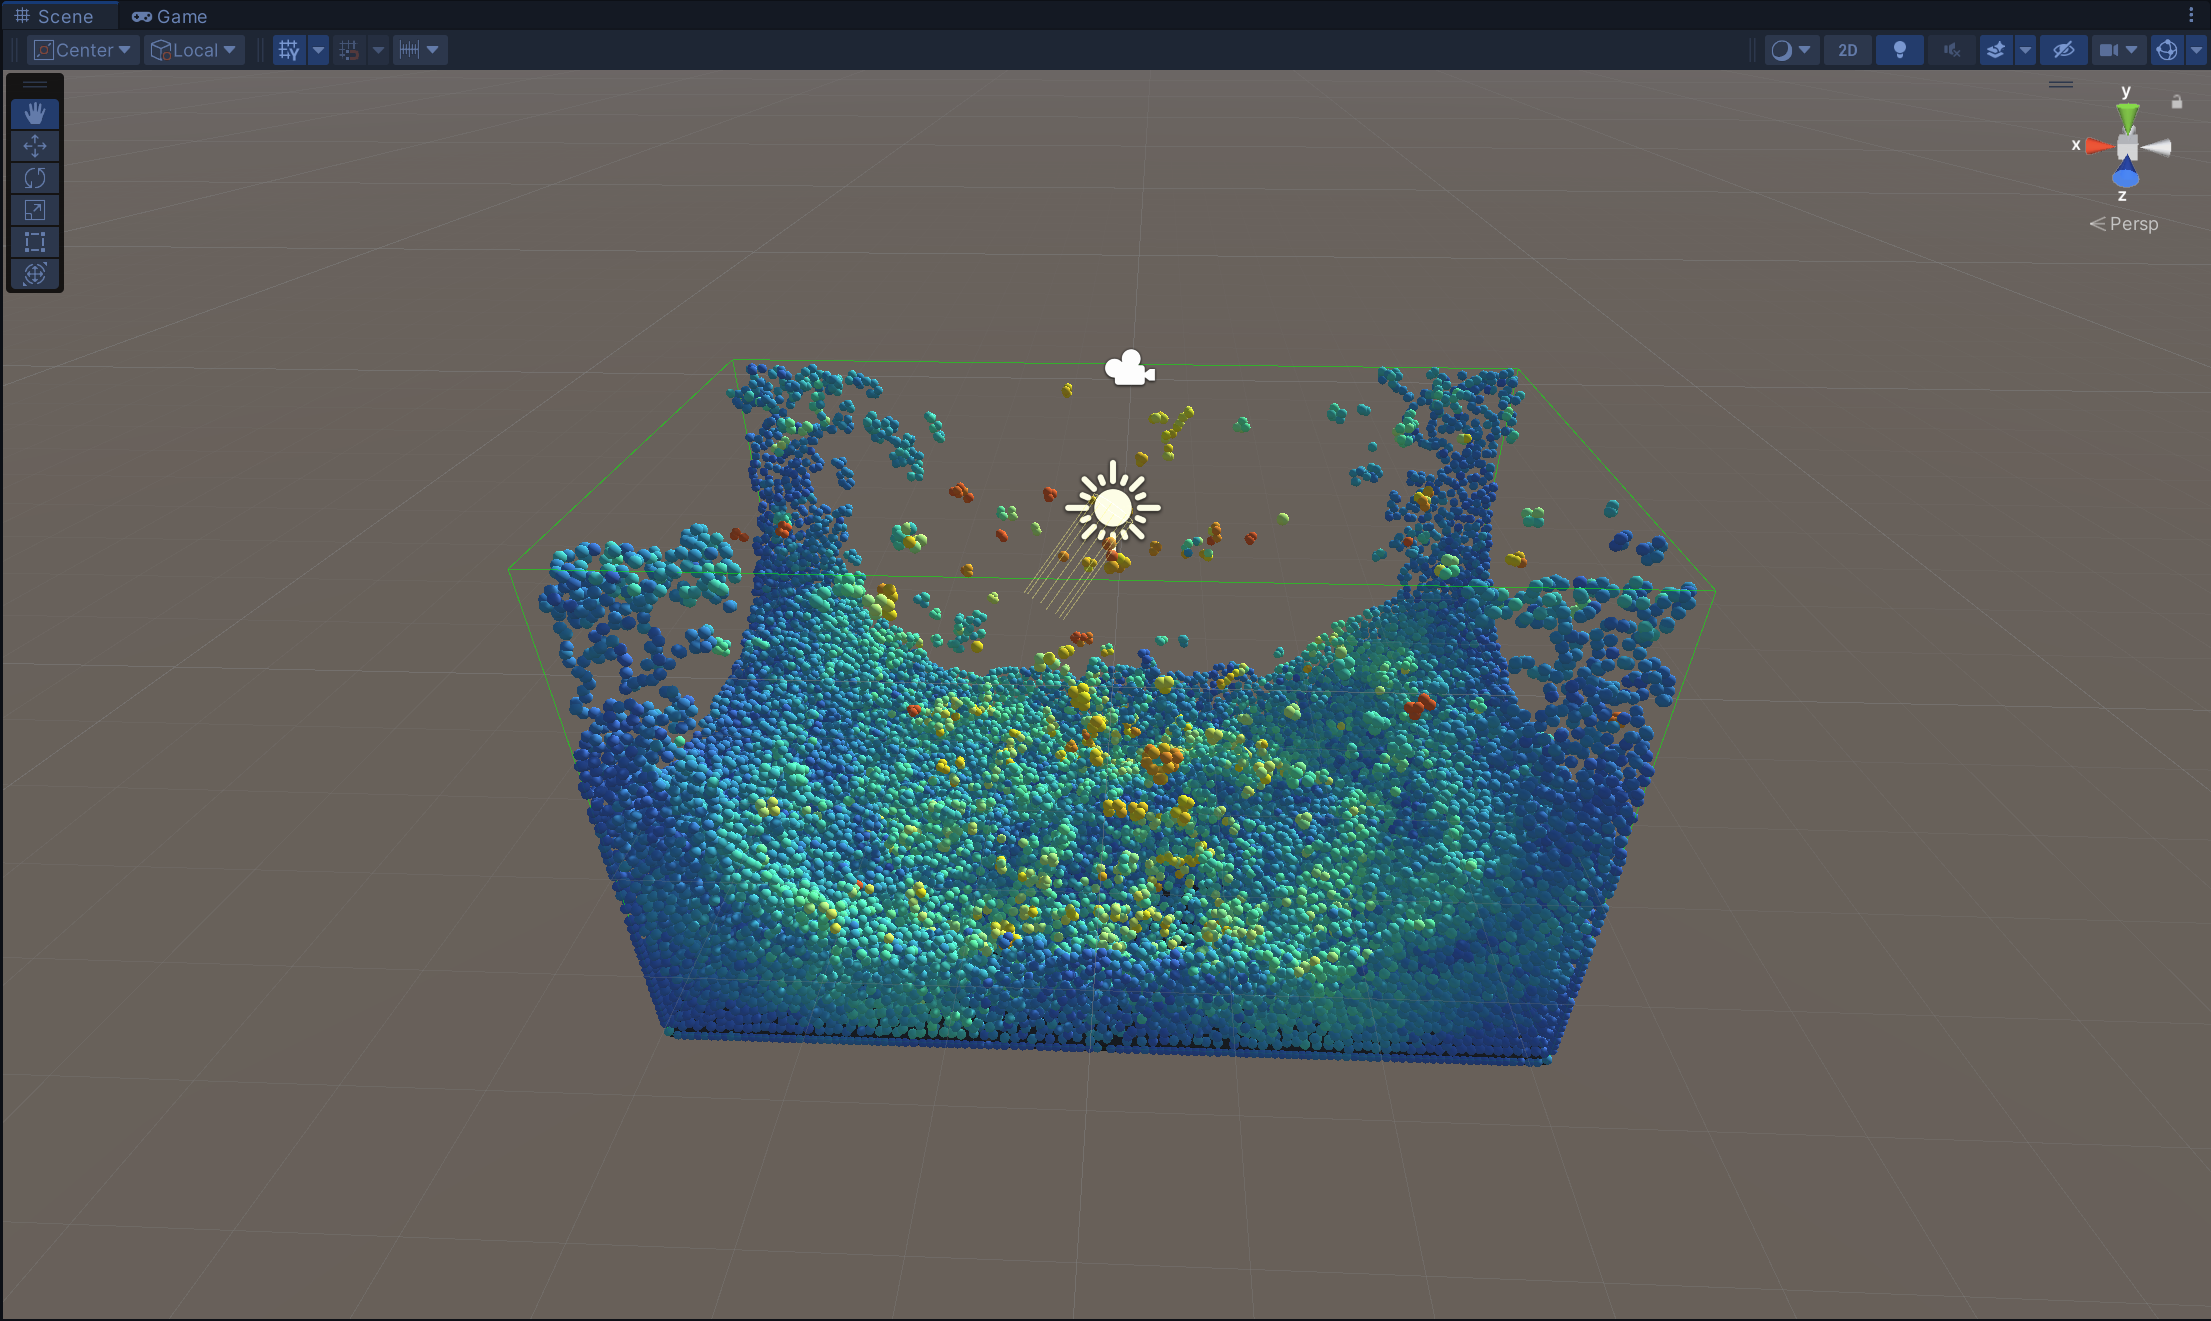
\includegraphics[width=0.9\textwidth]{water_model_mode.png}
        \caption{Water in Scene View}
        \label{fig:higher_velocity}
    \end{subfigure}%
    \hfill % Adds horizontal space between the subfigures
    \begin{subfigure}[b]{0.33\textwidth}
        \centering
        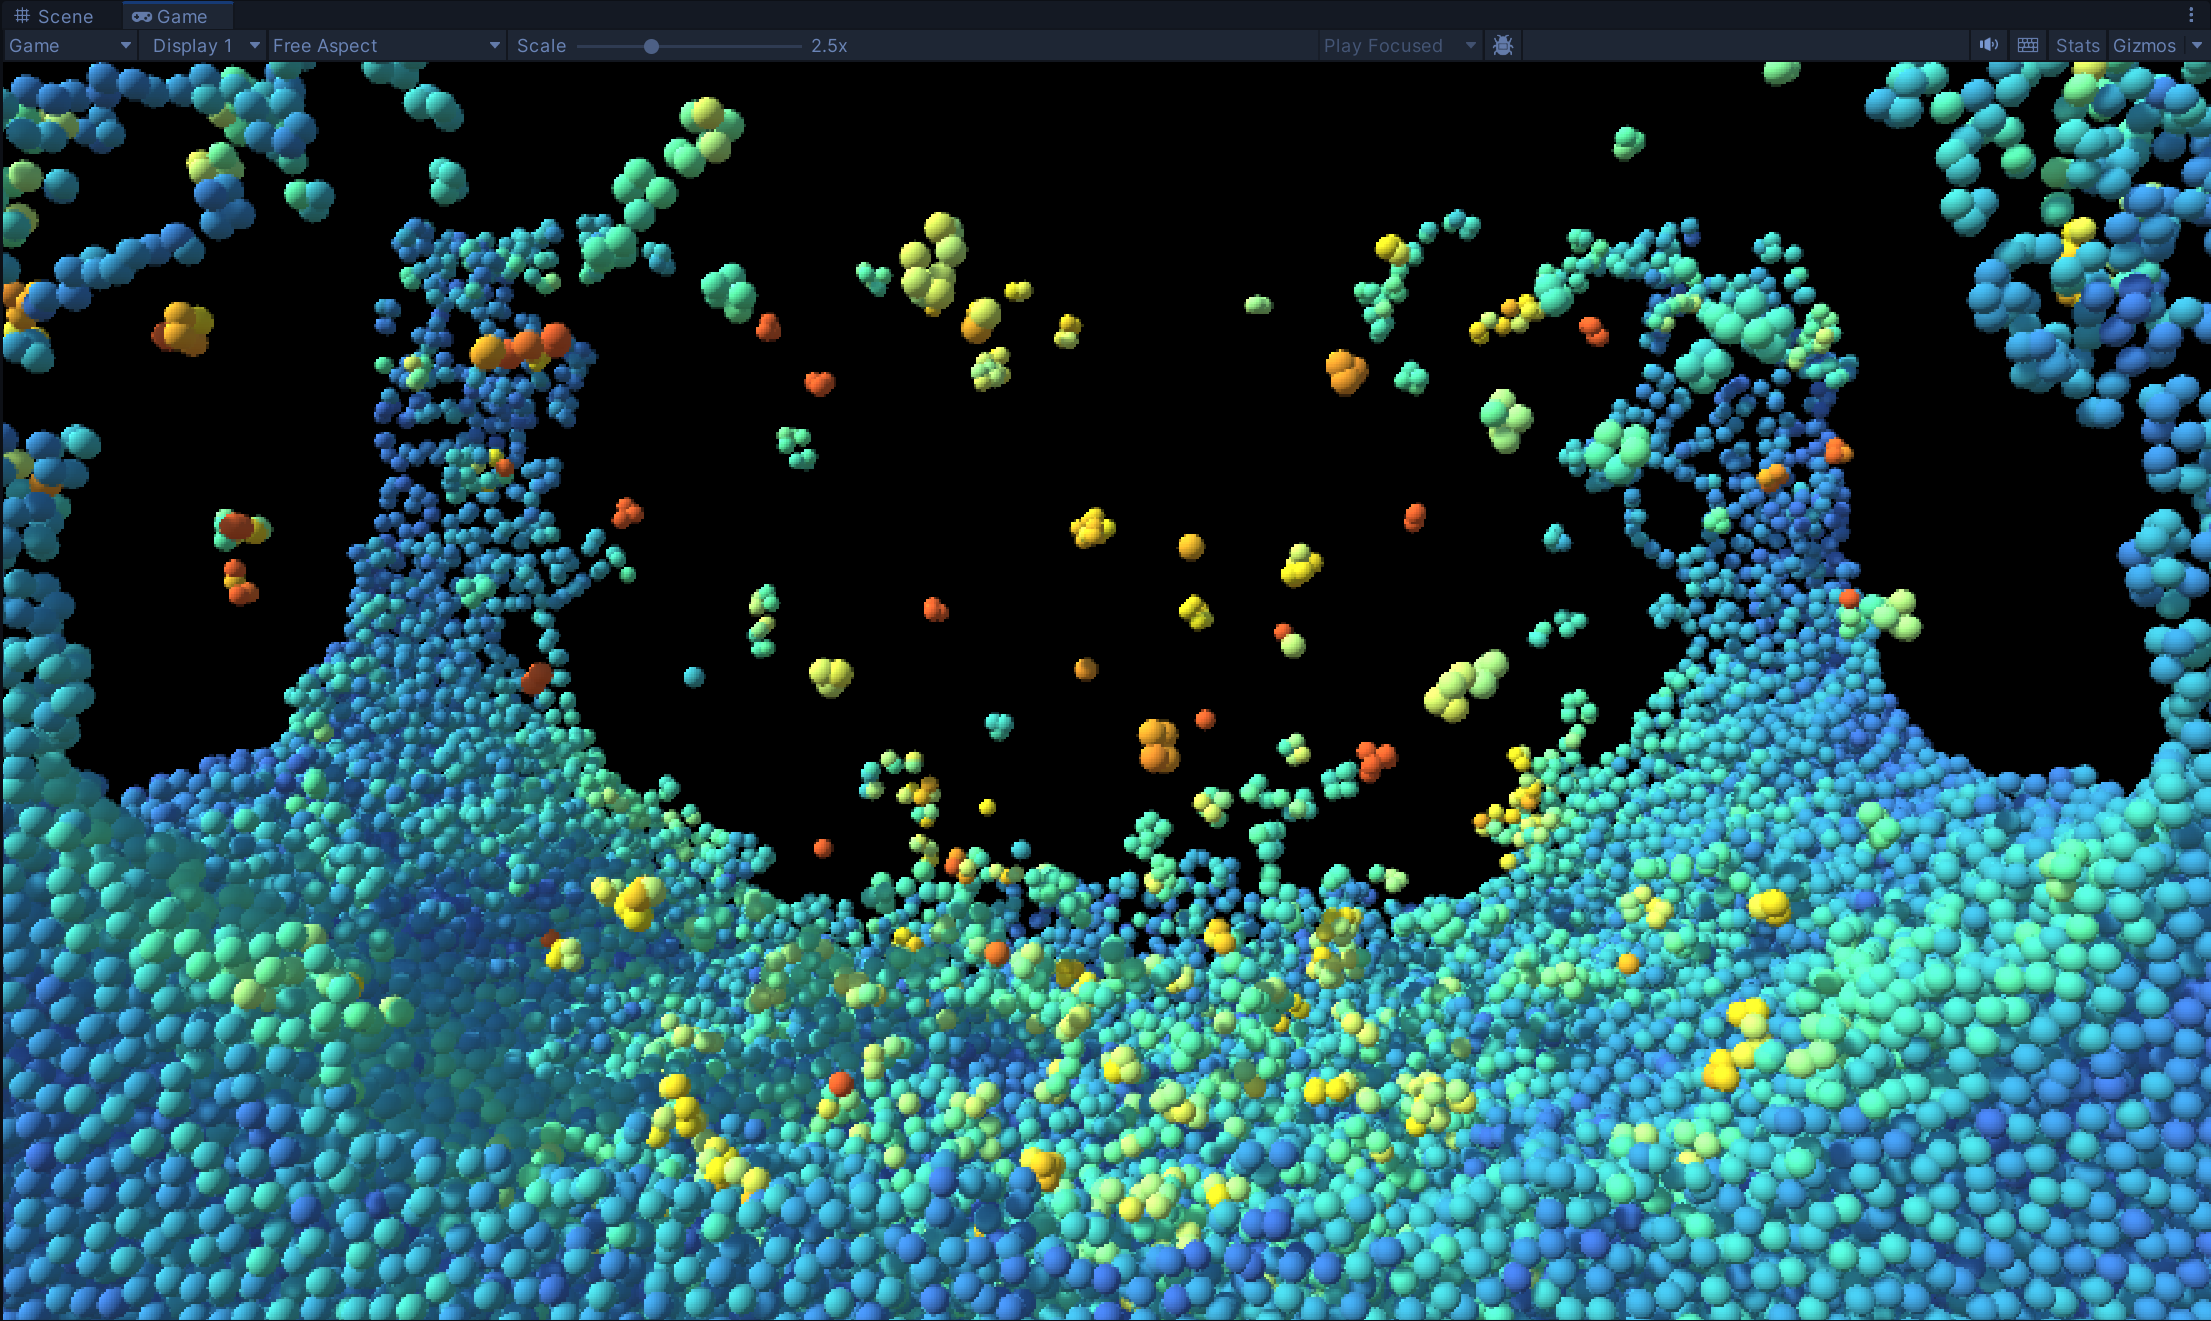
\includegraphics[width=0.9\textwidth]{water_game_mode.png}
        \caption{Water in Game Mode}
        \label{fig:lower_velocity}
    \end{subfigure}
        \begin{subfigure}[b]{0.33\textwidth}
        \centering
        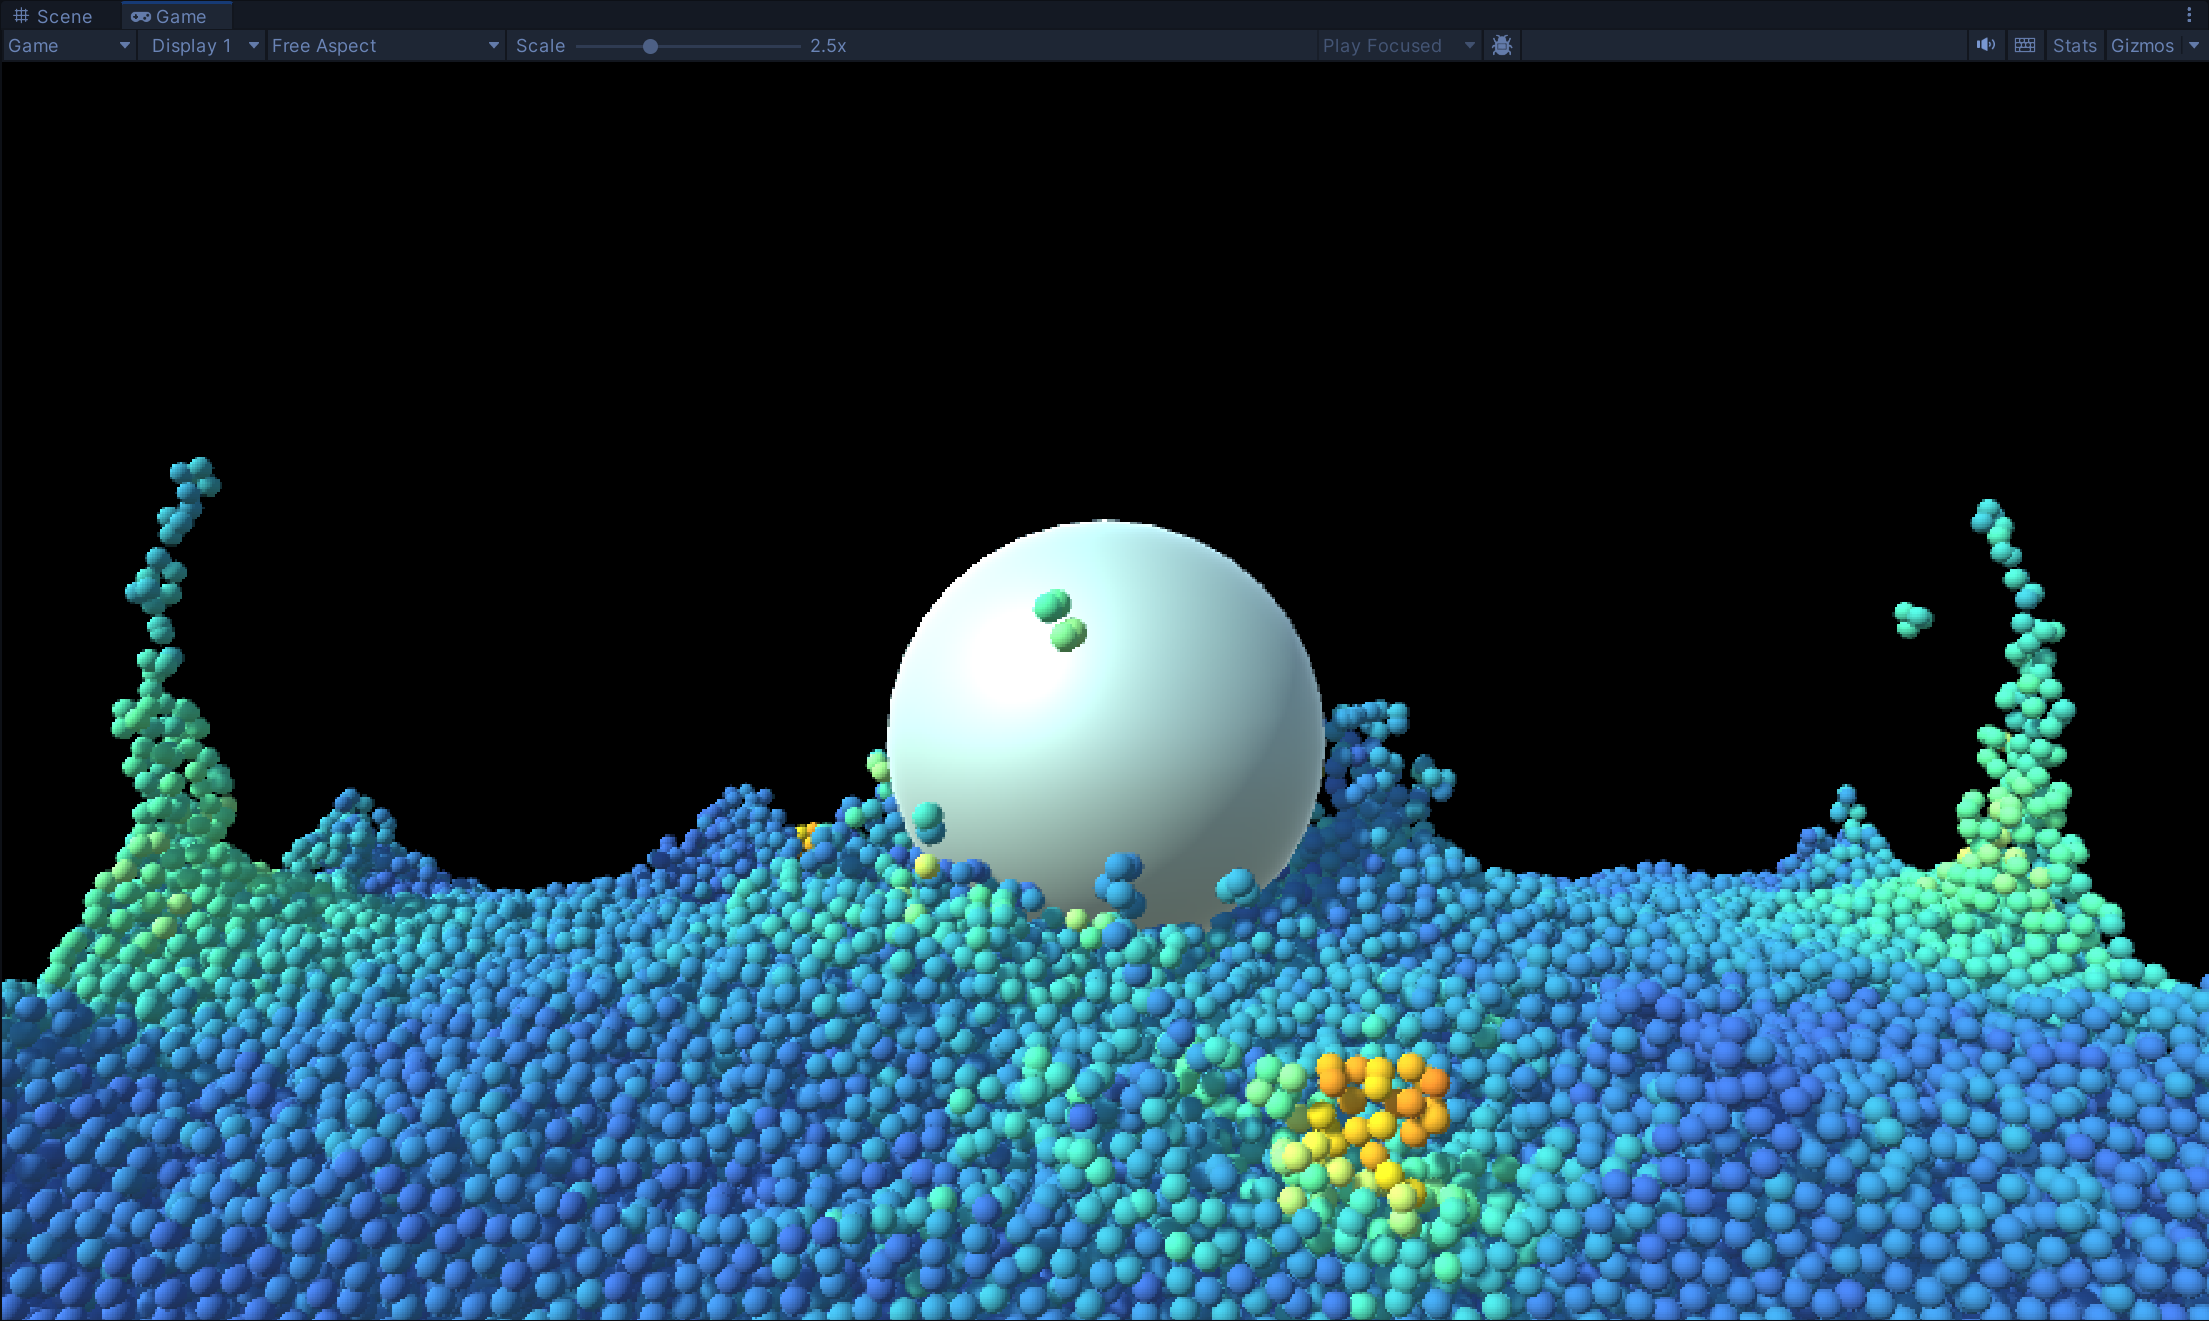
\includegraphics[width=0.9\textwidth]{ball_water.png}
        \caption{Ball drops in Water}
        \label{fig:lower_velocity}
    \end{subfigure}
\end{figure}

\section{Reflection}
\hspace*{1em} The above figures are preliminary simulation demos for the fluid and its interaction with the ball. More refinement is needed, for example, as seen in the figure, the scenario when liquid drops splashed out is not real. 
\noindent\hspace*{1em} In addition, we current simulate the fluid in the form of discrete liquid drops, just like those "ocean balls" in children's amusement parks. We will further make the simulation of fluid more real.

% Figure 3: water with tuned parameters



% \section{Introduction}

% \urllink{Overleaf}{https://www.overleaf.com/} is popular online \LaTeX{}
% editor. It can generate PDF files 
% without need to install a local \TeX{} distribution. Unfortunatelly, it doesn't
% support conversion to HTML out of the box. To get the HTML version of the
% document, we must use some tricks.

% There are many tools that support the conversion from \LaTeX{} to HTML, each of
% them use a different approach. I am a developer of
% \urllink{\TeX4ht}{https://tug.org/tex4ht/}, so I will present solution that
% uses this tool. 

% \TeX4ht uses \TeX{} for the actual conversion. It loads special configuration
% files for internal \LaTeX{} code or for the used packages. These configuration
% files patch commands with special instructions that insert HTML (or other
% supported formats). Because it uses \TeX{} for the actual conversion, it
% supports custom commands. It also supports font changing commands, so  it
% doesn't need custom configurations in many cases.

% The first method that use \TeX4ht for the conversion was presented by LianTze
% Lim. It uses a custom build file for
% \urllink{Latexmk}{https://www.overleaf.com/latex/examples/testing-html-export-with-tex4ht/rqcknjvwyyry} 
% that calls \TeX4ht. The downside is that the generated HTML file is not easilly accessible.  

% To make the conversion easier, I've set up \urllink{Docker image}{https://hub.docker.com/repository/docker/michalh21/make4ht-docker/general} for \TeX4ht. 
% Thanks to \urllink{GitHub Actions}{https://help.github.com/en/actions/automating-your-workflow-with-github-actions/about-github-actions}, 
% it is possible to use this image for the conversion of the Overleaf document to HTML. 
% The generated files can be published on the web using Github Pages, where they can be automatically 
% updated on every document change. This document is an example of this setup.

% \section{Setup}

% \subsection{On Overleaf}

% First step is to sync your Overleaf project with your GitHub account, following \foothref{a guide on 
%   Overleaf}{https://www.overleaf.com/learn/how-to/How_do_I_connect_an_Overleaf_project_with_a_repo_on_GitHub,_GitLab_or_BitBucket\%3F}
% {\texttt{https://www.overleaf.com/learn/how-to/How\_do\_I\_connect\_an\_Overleaf\_project\_with\_a\allowbreak\_repo\_on\_GitHub,\_GitLab\_or\_BitBucket\%3F}}. 
% Don't forget to run the \cmdname{Sync -> GitHub} command from Overleaf main menu every time you had updated the document.

% \subsection{On GitHub}
% Next step is to configure actions in the Github project created for your
% document. Two steps are necessary -- first  one compiles the document to HTML
% using \TeX4ht, the second step publishes the generated HTML files on the Web
% using \urllink{GitHub Pages}{https://pages.github.com/}

% For the web publishing we  use the \verb|actions-gh-pages|
% \urllink{action}{https://github.com/peaceiris/actions-gh-pages}. 

% When the keys are set up, you can create the workflow file. Select the
% \cmdname{Actions} tab and click the \cmdname{Set up a workflow yourself}
% button. It will open an editor with a YAML file for the Action workflow.
% Replace it with the following content:

% % I am just testing if this command works in the container
% \AtEndEnvironment{lstlisting}{\relax}

% \begin{lstlisting}{yaml}
% name: CI
% on: [push]
% jobs:
%   build:
%     runs-on: ubuntu-latest
%     steps:
%     - uses: actions/checkout@v1
%     - name: Run make4ht
%       uses: docker://ghcr.io/michal-h21/make4ht-action:latest
%       env:
%         command: "make4ht -u -d out main.tex"
%     - name: Publish the web pages
%       uses:  peaceiris/actions-gh-pages@v3
%       with:
%         github_token: ${{ secrets.GITHUB_TOKEN }}
%         publish_dir: ./out
% \end{lstlisting}

% The important part of the configuration is the \cmdname{command} key. It
% contains the actual command used for the compilation. We use
% \urllink{Make4ht}{https://ctan.org/pkg/make4ht?lang=en}, build system for
% \TeX4ht.

% Command \verb|"make4ht -u -d out main.tex"| creates UTF-8 encoded HTML file
% from the \cmdname{main.tex} input file. The \texttt{-d} option specifies the
% output directory for the HTML files. This directory will be used for the web
% publishing and should be passed to the \verb|publish_dir| key in
% \textit{Publish the web pages} step.

% The web will be published at \url{https://yourgitubusename.github.io/project_name/main.html}. 
% \section{Links}
% \begin{itemize}
%     \item This document: \url{https://www.kodymirus.cz/overleaf-html-sample/main.html}
%     \item Source repository: \url{https://github.com/michal-h21/overleaf-html-sample} 
% \end{itemize}
 



\end{document}
